%!TEX root = ../../super_main.tex

\section{Data Usefulness}
\label{sec:data_usefulness}

We need to investigate if it is possible to use the uMiner platform to gather snapshots and if the snapshots are actually useful for some reality mining related task, e.g. by creating some context aware application. We have for this reason created a simple campaign, that asks the participants if their phone is placed on the table or not, corresponding to the specification shown in \tabref{tab:phone_placement_campaing}.

\begin{table}[!htbp]
    \centering
    \begin{tabular}{|m{0.34\textwidth}|m{0.6\textwidth}|} 
  \hline
  \textbf{Snapshot per Campaign}    & 30 snapshots      \\ \hline
  \textbf{Samples per Snapshot}     & 1 samples         \\ \hline
  \textbf{Sample delay}             & 4000 ms           \\ \hline
  \textbf{Measurement per Sample}   & 30 measurements   \\ \hline
  \textbf{Measurement delay}        & 200 ms            \\ \hline
  \textbf{Sensors}                  & \begin{itemize}[noitemsep]
                \item Accelerometer 
                \item Compass
                \item Gyroscope
              \end{itemize}                             \\ \hline
    \textbf{Questions}                & \begin{itemize}[noitemsep]
                                            \item Was the phone placed on the table?
                                        \end{itemize} \\ \hline
    \end{tabular}
    \caption{Phone placement campaign.}
    \label{tab:phone_placement_campaing}
\end{table}

This configuration results in snapshots with a duration of 10 seconds. Note that it is not an intended use case to have 10 seconds, because a question every 10th seconds is simply too intrusive for the participants in an everyday scenario. We have furthermore specified, that we want 30 snapshots from this campaign, which means the participants of this campaign will be monitored for a 5 minute period in total. We have created this dense campaign, because we wanted to get some snapshots, with which we could quickly determine if the collected data is useful for creating some context aware application. The snapshots from this data was used to create an example application called \emph{Where Am I?}, which guesses if the device is placed on the table or in a pocket, as seen in \figref{fig:where_am_i_app}.

\begin{figure}[!htbp]
    \centering
    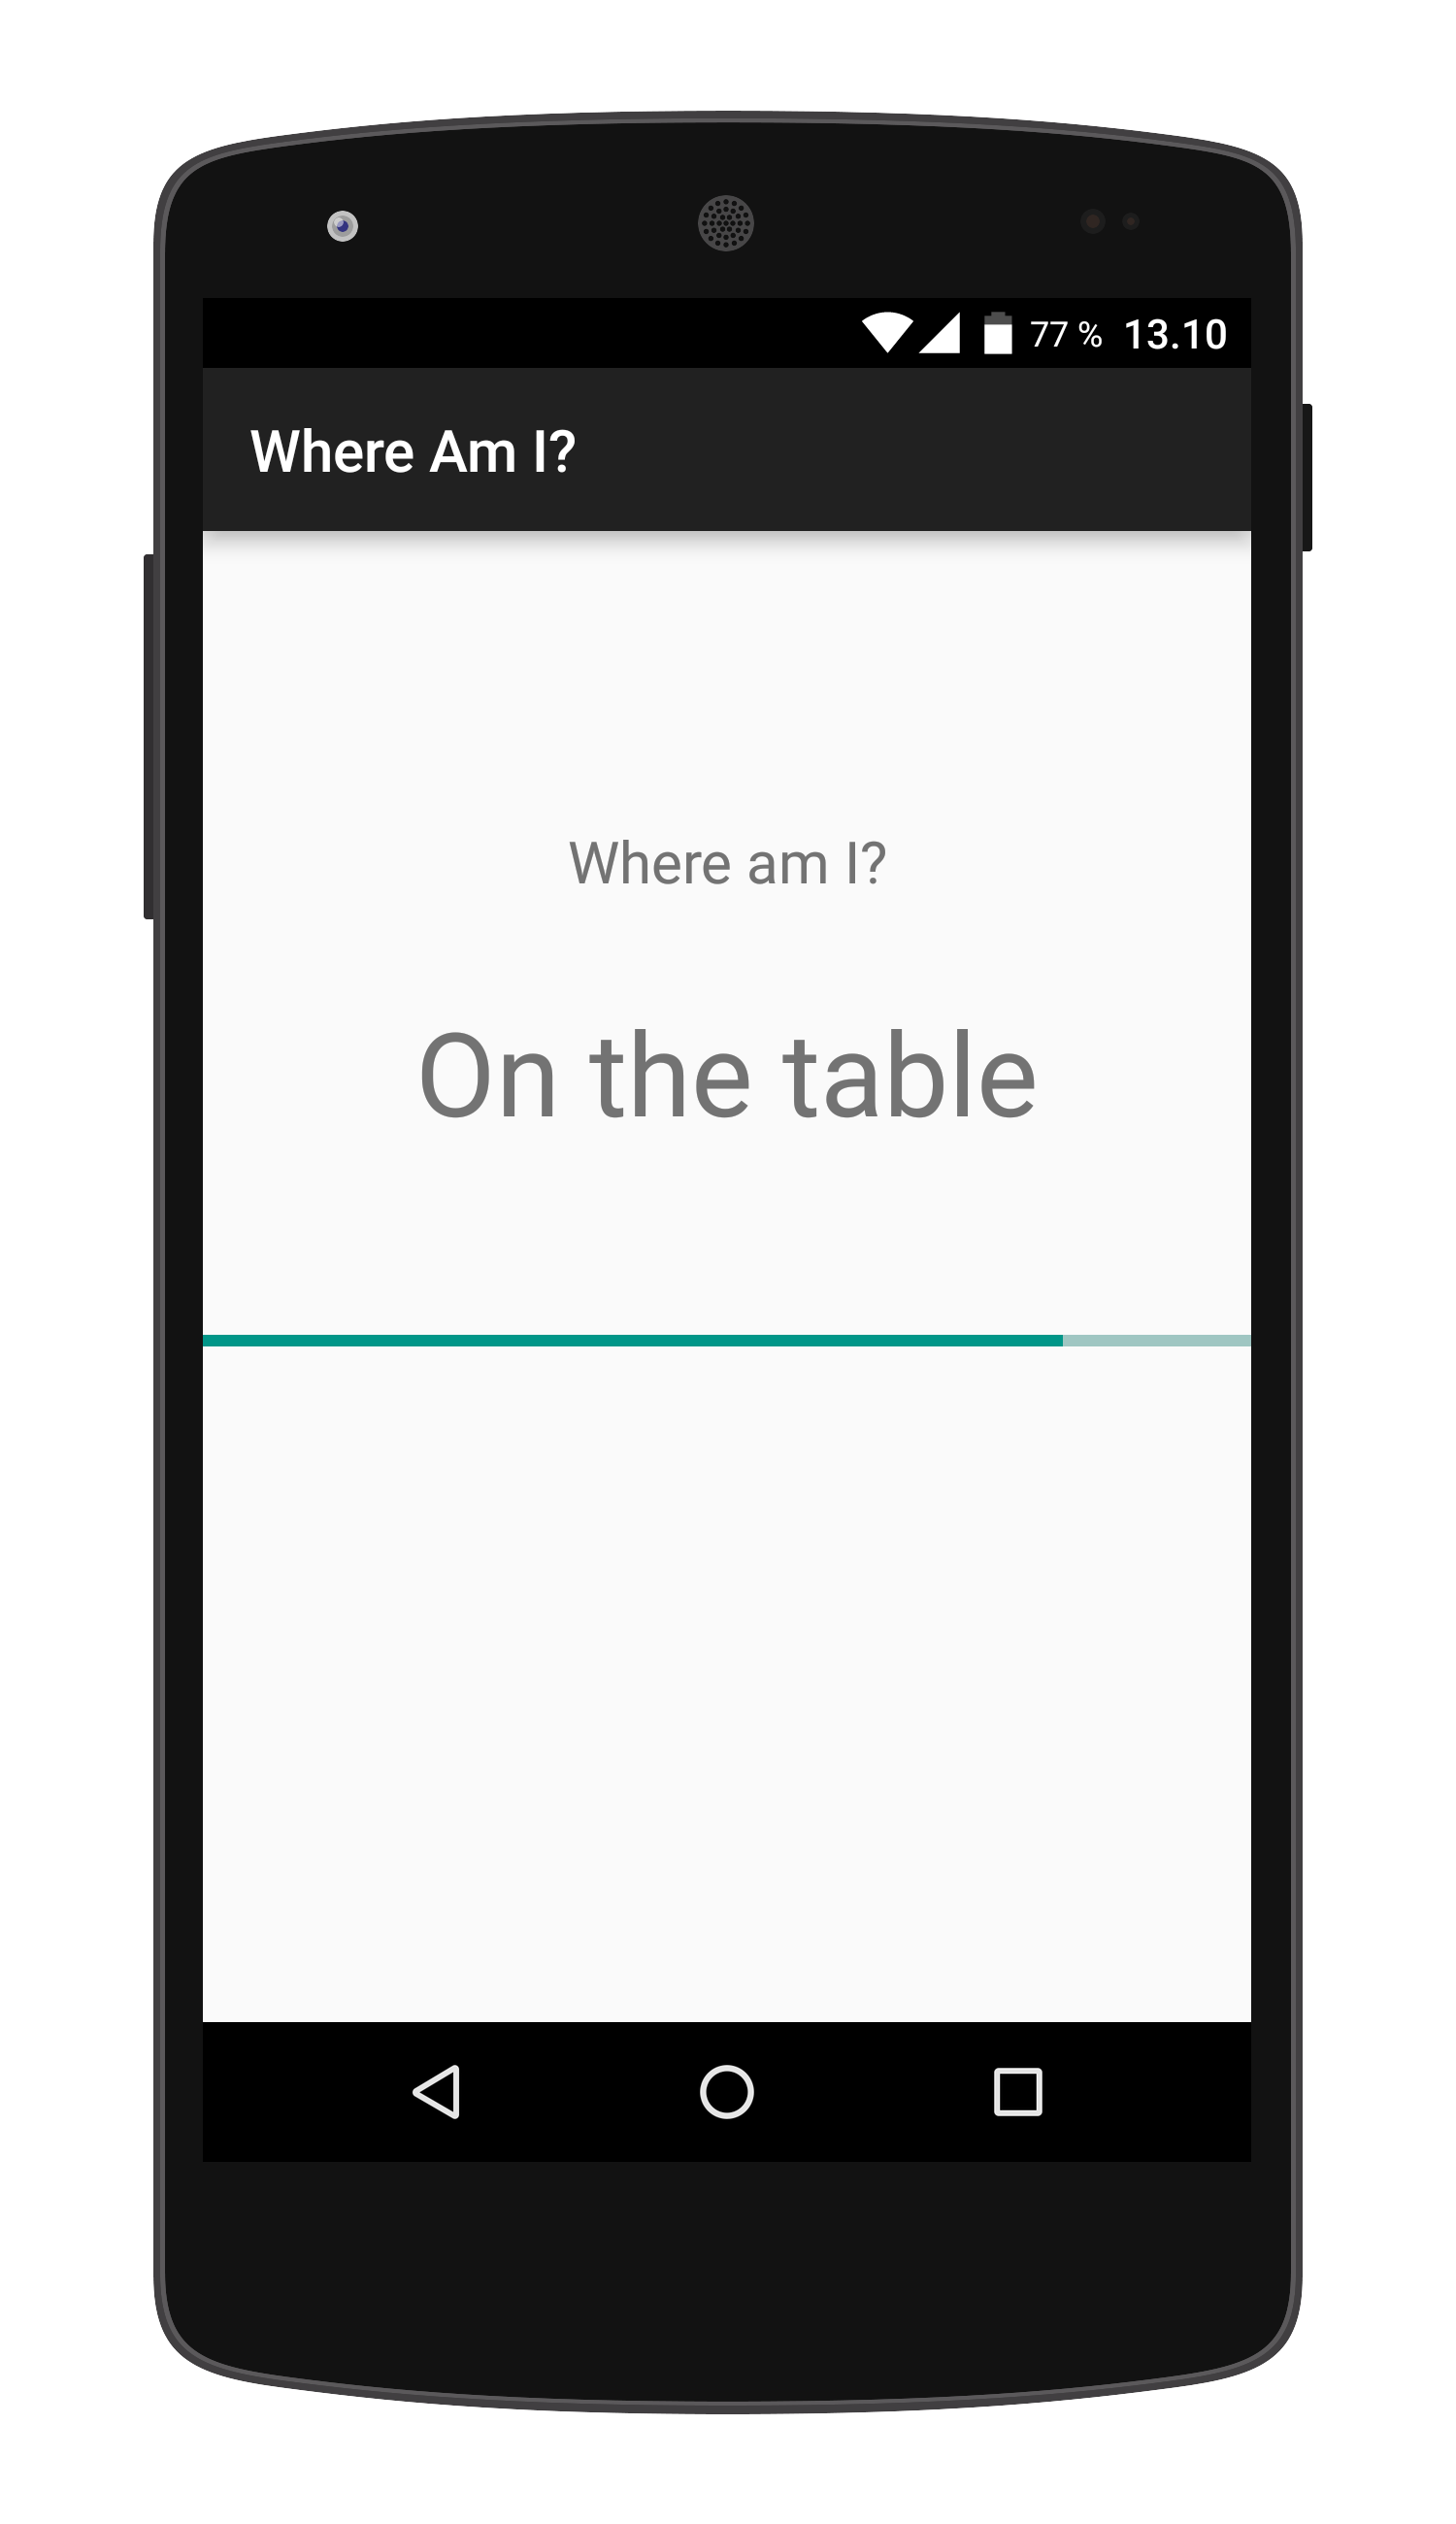
\includegraphics[width=.35\textwidth ]{graphic/quality_assurance/where_am_i_app.png}
    \caption{The example \emph{Where Am I?} application.}
    \label{fig:where_am_i_app}
\end{figure}
\FloatBarrier

The \emph{Where Am I?}-application continuously guesses if the phone is placed on a table or not, using an underlying Naïve Bayes classifier. This application starts up, trains the classifier using the snapshots, and then predicts, in real time, the placement of the phone. This classifier was implemented using a library called WEKA\footnote{https://weka.wikispaces.com/}, which has some predefined methods and data types that makes it relatively easy to implement a Naïve Bayes classifier, The gathering of sensor values was implemented using sensor providers from uMiner.
\\\\
We found it pretty effortless, to implement an application that has some notion of the context in which it exist, given our snapshots and the WEKA machine intelligence library. We spend roughly 16 man hours on the creation and execution of a campaign, and on implementing features that allow this application to parse the gathered snapshots, train a model, and display the prediction in a simple interface.